\documentclass{beamer}

\mode<presentation> {
  \usetheme{Warsaw}
  \setbeamercovered{transparent}
  \setbeamertemplate{itemize items}[default]
  \setbeamertemplate{enumerate items}[default]
  \setbeamertemplate{navigation symbols}{} %no nav symbols
}

\usepackage{ucs}
\usepackage[utf8x]{inputenc}
\usepackage[czech]{babel}
\usepackage{palatino}
\usepackage{graphicx}
\usepackage[absolute,overlay]{textpos}
\usepackage{verbatim}
\usepackage{hyperref}
\hypersetup{
  unicode=true,
  pdfsubject={ReReSearch},
  pdfkeywords={KNOT Group FIT VUT, ReReSearch}
}


%------------------------------------------------------------------------------
\title[ReReSearch, KNOT Group, FIT VUT\hspace{9em}\insertframenumber/
\inserttotalframenumber]{ReReSearch}
\subtitle[KNOT Group]{Výzkumná skupina znalostních technologií}
\author{Stanislav Heller, xhelle03@stud.fit.vutbr.cz}
\institute[FIT VUT]{
  Fakulta Informačních Technologií\\
  Vysoké Učení Technické v Brně
}
\date{7.~2.~2013}
%------------------------------------------------------------------------------


\begin{document}

\begin{frame}
  \titlepage
\end{frame}

\begin{frame}
  \frametitle{Obsah}
  \tableofcontents
\end{frame}


% -----------------------------------------------------------------------------
% NLP Group
% -----------------------------------------------------------------------------
\section{KNOT Group}

\begin{frame}
  \frametitle{Výzkumná skupina znalostních technologií}
  \begin{itemize}
    \item jedna z mnoha výzkumných skupin na FIT
    \item vedení: doc. Smrž
    \item z hlediska fakulty spadá pod UPGM (ústav počítačové grafiky a multimédií)
    \item nemá žádnou místnost, je to abstraktní organizace
  \end{itemize}
\end{frame}

\begin{frame}
  \frametitle{Co děláme}
  \begin{itemize}
    \item strukturní jazykové modely, syntaktická analýza
    \item technologie sémantického webu
    \item extrakce dat z textových dokumentů a z webu, dolování znalostí
    \item spolupráce s oblastí biomedicíny (projekt M-eco)
  \end{itemize}
\end{frame}

\begin{frame}
  \frametitle{Proč pracovat u nás}
  \begin{itemize}
    \item nové metody, nástroje
    \item možnost pracovat na nových technologiích
    \item praxe - mimoškolní projekty
    \item zlepšení programátorských a analytických schopností
    \item náměty na bakalářské a diplomové práce
    \item zajímavé finanční ohodnocení (pozn. srovnání)
  \end{itemize}
\end{frame}

\begin{frame}
  \frametitle{Pravidla}
  \begin{itemize}
    \item škola? ne! výzkum!
    \item spolupráce: maily, schůzky
    \item využití výzkumných serverů pro výzkumné účely
    \item veškerý software a data je zakázáno používat mimo účely KNOT
    \item při nečinnosti navrácení peněz
    \item možnost snížení aktivity při dokončování projektů a ve zkouškovém
  \end{itemize}
\end{frame}

\begin{frame}
  \frametitle{Povinnosti}
  \begin{itemize}
    \item {\alert{práce}}
    \item KNOT IS / týdenní výkazy, hodiny k odpracování
      \begin{itemize}
        \item \textcolor{blue}{\underline{\href{http://knot.fit.vutbr.cz/knotis/}{http://knot.fit.vutbr.cz/knotis/}}}
      \end{itemize}
    \item dokumentace: wiki, README, generovaná dokumentace
    \item slušné chování, odpovídání na maily
    \item dodržování štábní kultury projektu
  \end{itemize}
\end{frame}

\begin{frame}
  \frametitle{Dotazy k KNOT Group}
  { ? }
\end{frame}


% -----------------------------------------------------------------------------
% Citacni databaze
% -----------------------------------------------------------------------------

\section{Cita{\v{c}}n\'{i} databáze}

\begin{frame}
  \frametitle{Citační databáze - úvod do problematiky}
  \begin{itemize}
    \item Co je citační databáze?
      \begin{itemize}
        \item systém pro shromažďování dat o vědeckých publikacích
        \item umožňuje vyhledávání publikací a autorů podle různých parametrů (citovanost..)
        \item nejčastěji webová služba
        \item CiteSeerX, Google Scholar, Mendeley, DBLP, Elsevier
      \end{itemize}
    \item Využití
      \begin{itemize}
        \item získávání informací o nejnovějších metodách v různých vědeckých disciplínách, aktuální směr výzkumu, trendy
        \item pro IT: nové metody, algoritmy, teorie...
      \end{itemize}
  \end{itemize}
\end{frame}

\subsection{Slovník}
\begin{frame}
  \frametitle{Slovník}
  \begin{description}
    \item[Publikace -] {kniha (book), časopis, sborník (journal), článek v časopise (article), 
                        DP (master thesis), disertační práce (phdthesis), výzkumná zpráva 
                        (deliverable), články}
    \item[Citace -]    {text (úsek) v publikaci, který je převzat z jiného zdroje. K citaci
                        patří její číslo odkazující na referenci}
    \item[Reference -] {patří k citaci. Je uvedena na konci dokumentu v literatuře.
                        Obsahuje název citované publikace, autory, kde byl
                        článek publikován a kdy, rozsah stran, případně odkaz na online
                        verzi publikace}
  \end{description}
\end{frame}

\begin{frame}
  \frametitle{Citace vs reference - příklad}
  \begin{block}{Citace}
    \textit{..it is a generalization of the Aubert's idea [13], who proved this property 
            for the isotropic diffusion tensor...}
  \end{block}

  \begin{block}{Reference}
     \textit{[13] G. Aubert and P. Kornprobst. Mathematical Problems in Image 
                    Processing: PDE’s and the Calculus of Variations, vol. 147 of 
                    App. Mathem. Sciences. Springer-Verlag, January 2002.}
  \end{block}
  {\textbf{Pozor!} Často se pod pojmem citace myslí reference!}
\end{frame}

\begin{frame}
  \frametitle{Slovník}
  \begin{description}
    \item[Anotace (annotation) -]   {stručný popis, který shrnuje a/nebo hodnotí daný zdroj 
                                     - současně komentuje jeho hodnotu nebo relevanci} \\
    \alert{\textbf{anotace \begin{math} \neq \end{math} abstrakt}}
    \item[Anotovaná bibliografie -] {sestava anotací k dokumentům určitého tématu}
    \item[Výzkumný projekt -] {projekt, který řeší netriviální problém. Výstupem je buď
                               nějaký program, zjištění, statistiky nebo seznam
                               doporučení (změny atp.). Projekt má řešitele a zadavatele. Je třeba
                               vydávat výzkumné zprávy}
    \item[Sociální citační systém -] {Connotea, CiteULike, Bibsonomy, Mendeley}
  \end{description}
\end{frame}

\begin{frame}
  \frametitle{Slovník}
  \begin{description}
    \item[Série konferencí -] {konference se stejným hlavním názvem konané každý rok}
    \item[Konference -] {událost, jíž se účastní výzkumníci, kteří zde prezentují své
                         nové myšlenky a publikace. Jednotlivý běh konference ze série}
    \item[Organizace -] {většinou nakladatelství nebo škola, kde byla publikace vydána.}
    \item[Sociální citační systém -] {Connotea, CiteULike, Bibsonomy, Mendeley}
  \end{description}
\end{frame}

\begin{frame}
  \frametitle{Příklady entit}
  \begin{block}{Série konferencí}
    The International Conference on Language Resources and Evaluation
  \end{block}

  \begin{block}{Konference}
    The sixth international conference on Language Resources and Evaluation (LREC 2008)
  \end{block}

  \begin{block}{Organizace}
    Springer US, IEEE Press, FIT BUT
  \end{block}
\end{frame}

\subsection{Existující systémy}
\begin{frame}
  \frametitle{Existující citační databáze}
  \begin{itemize}
    \item {\textbf{Google Scholar -} vyhledávání publikací}
      \begin{itemize}
        \item \textcolor{green!50!black}{zdarma, pohodlné vyhledávání, jazykově neomezené}
        \item \textcolor{red}{analýza citací, stahování, neobsahuje konference, organizace}
      \end{itemize}
    \item {\textbf{CiteSeerX -} vyhledávání publikací včetně PDF verzí}
      \begin{itemize}
        \item \textcolor{green!50!black}{zdarma, pohodlní vyhledávání}
        \item \textcolor{red}{prakticky výhraně EN}
      \end{itemize}
    \item {\textbf{DBLP -} 1,6 mil. článků, konference, sborníky, knihy}
      \begin{itemize}
        \item \textcolor{green!50!black}{zdarma, dostupná data v XML}
        \item \textcolor{red}{analýza citací}
      \end{itemize}
  \end{itemize}
\end{frame}

\begin{frame}
  \frametitle{Existující citační databáze}
  \begin{itemize}
    \item {\textbf{Mendeley -} sociální citační systém}
      \begin{itemize}
        \item \textcolor{green!50!black}{zdarma, velká databáze} 
        \item \textcolor{red}{autoři nejsou entita}
      \end{itemize}
    \item {\textbf{Microsoft Academic Search -} 37 mil. článků}
      \begin{itemize}
        \item \textcolor{green!50!black}{zdarma, vyhledávání, kvalitní analýza citací,
                                         mnoho entitních množin, zahrnuje organizace atp.} 
        \item \textcolor{red}{?}
      \end{itemize}
    \item {\textbf{Scopus (Elsevier)}}
      \begin{itemize}
        \item \textcolor{green!50!black}{citační analýza, konference}
        \item \textcolor{red}{nezahrnuje knihy, kapitoly}
      \end{itemize}
  \end{itemize}
\end{frame}

\begin{frame}
  \frametitle{Problémy existujících citačních databází}
  \begin{itemize}
    \item stále jen citační databáze s malou inteligencí
      \begin{itemize}
        \item automatické navrhování vhodných dokumentů k dané tématice
        \item sémantická blízkost dokumentů
        \item automatické zhodnocení výsledků: \textit{"neděláš to špatně, ale ostatní to dělají na daleko větší trénovací množině"}
      \end{itemize}
    \item malé množství entitních množin
    \item nikdo se nezajímá o vědecké projekty, geografické údaje atp.
  \end{itemize}
\end{frame}


\begin{frame}
  \frametitle{Dotazy k tematice citačních databází}
  {?}
\end{frame}


% -----------------------------------------------------------------------------
% ReReSearch
% -----------------------------------------------------------------------------
\section{Projekt ReReSearch}

\begin{frame}
  \frametitle{Projekt ReReSearch [RRS]}
  \begin{itemize}
    \item ne jen citační databáze
    \item {\textbf{získávání dat:} extrace (publikace, konference, vědci, projekty)}
    \item {\textbf{analýza:} získávání znalostí, sledování trendů}
    \item {\textbf{rozhraní:} vyhledávač, odpovídání na otázky, generování portálů}
  \end{itemize}
  \begin{block}{Cíle}
    \begin{itemize}
      \item vybudovat znalostní systém o výzkumu a vědě
      \item přidat inteligentní funkcionalitu
      \item systém musí sám "žít" a hledat si informace
      \item \textbf{RRS musí řešit problémy současných databází}
    \end{itemize}
  \end{block}
\end{frame}

\subsection{Architektura}
\begin{frame}
  \frametitle{RRS: architektura}
  \begin{itemize}
    \item ReReSearch =
      \begin{itemize}
        \item databáze (PostgreSQL) +
        \item řídící systém (neexistuje) +
        \item výkonné moduly == vaše projekty +
        \item rozhraní
      \end{itemize}
    \item athena3:/mnt/data2/reresearch/
    %\item \textcolor{blue}{\underline{\href{http://athena3.fit.vutbr.cz:30101/databrowser/}{http://athena3.fit.vutbr.cz:30101/databrowser/}}}
  \end{itemize}
\end{frame}

\begin{frame}
  \frametitle{RRS: architektura}
  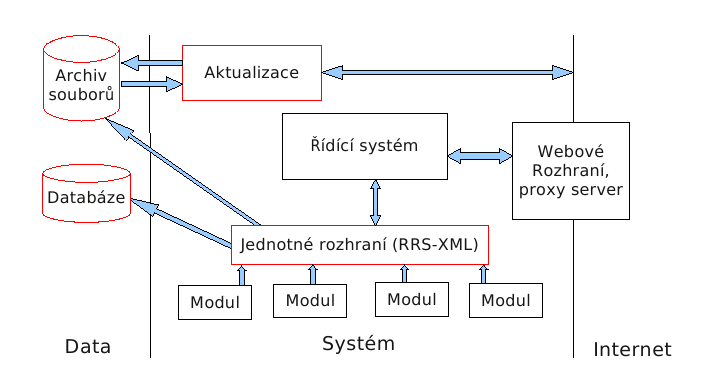
\includegraphics[width=10cm]{rrs_arch.png}
\end{frame}

\subsection{Databáze}
\begin{frame}
  \frametitle{RRS: databáze}
  \begin{itemize}
    \item PostgreSQL
    \item přístup
      \begin{itemize}
        \item psql
        \item Python - psycopg2
        %\item PhpPgAdmin - \textcolor{blue}{\underline{\href{http://athena3.fit.vutbr.cz:30101/phppgadmin/}{http://athena3.fit.vutbr.cz:30101/phppgadmin/}}}
        \item \textcolor{blue}{\underline{\href{https://merlin.fit.vutbr.cz/nlp-wiki/index.php/Rrs\_db}{https://merlin.fit.vutbr.cz/nlp-wiki/index.php/Rrs\_db}}}
      \end{itemize}
  \end{itemize}
\end{frame}

\begin{frame}
  \frametitle{DB: přehled entitních množin (redukovaný)}
  \begin{itemize}
    \item publication, person, event, project, organization, reference, citation, presentation
    \item text, url, file, network, language, award, contact, topic, keyword, tag, 
    \item location - geografická ontologie
  \end{itemize}
\end{frame}


\begin{frame}
  \frametitle{DB: publikace (publication)}
  \begin{columns}
    \column{.7\textwidth}
      \fontsize{10pt}{11pt}\selectfont
      \begin{itemize}
        \item název, normalizovaný tvar názvu, zkratka, 
        \item jazyk, typ, série, mateřská publikace, počet stran
        \item "submitted" - přihlášené k vydání, událost, kde byla publikace prezentována
        \item prezentace kde byla publikace prezentována, vydavatel a další
        \item text, ke kterému se váže (z hlediska databáze je to fulltext, string)
        \item DOI, ISBN, ISSN, vydání, číslo svazku, datum vydání, abstrakt
      \end{itemize}
    \column{.3\textwidth}
      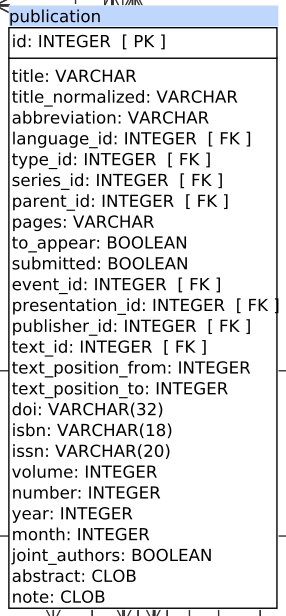
\includegraphics[width=2.5cm]{rrs_db_publ.jpeg}
  \end{columns}
\end{frame}

\begin{frame}
  \frametitle{DB: osoba - autor/editor/vedoucí (person)}
  \begin{columns}
    \column{.7\textwidth}
      \begin{itemize}
        \item křestní jméno, prostřední jméno, příjmení
        \item celé jméno, celé jméno v ASCII (bez diakritiky)
        \item celé jméno v národní formě (v národním jazyce)
        \item pohlaví
      \end{itemize}
    \column{.3\textwidth}
      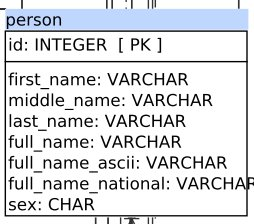
\includegraphics[width=2.5cm]{rrs_db_pers.jpeg}
  \end{columns}
\end{frame}

\begin{frame}
  \frametitle{DB: organizace (organization)}
  \begin{columns}
    \column{.4\textwidth}
      \fontsize{9pt}{11pt}\selectfont
      \begin{itemize}
        \item typ, rodičovská organizace (např. vztah univerzita-fakulta-ústav)
        \item lokace (tam, kde organizace sídlí)
        \item název, normalizovaný název
        \item organizace může mít jeden oficiální název a mnoho neoficicálních (tabulka organization\_name)
      \end{itemize}
    \column{.6\textwidth}
      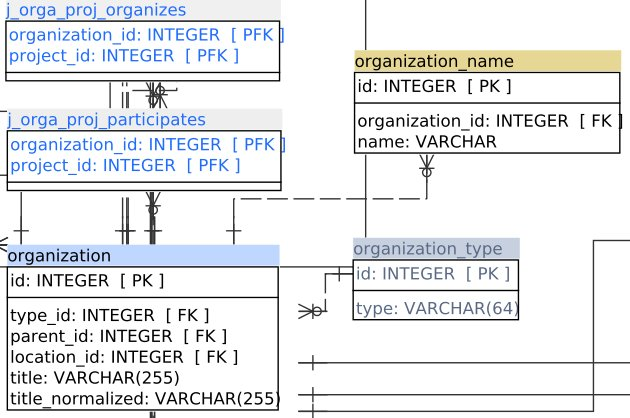
\includegraphics[width=6cm]{rrs_db_orga.jpeg}
  \end{columns}
\end{frame}

\begin{frame}
  \frametitle{DB: událost - konference/workshop/... (event)}
  \begin{columns}
    \column{.5\textwidth}
      \fontsize{10pt}{11pt}\selectfont
      \begin{itemize}
        \item typ, série (!!), rodičovská událost (vztah např. konference - přidružený workshop)
        \item název, normalizovaný název, zkratka, 
        \item číslo události (např. pořadí konference v rámci série)
        \item časy OD - DO
      \end{itemize}
    \column{.5\textwidth}
      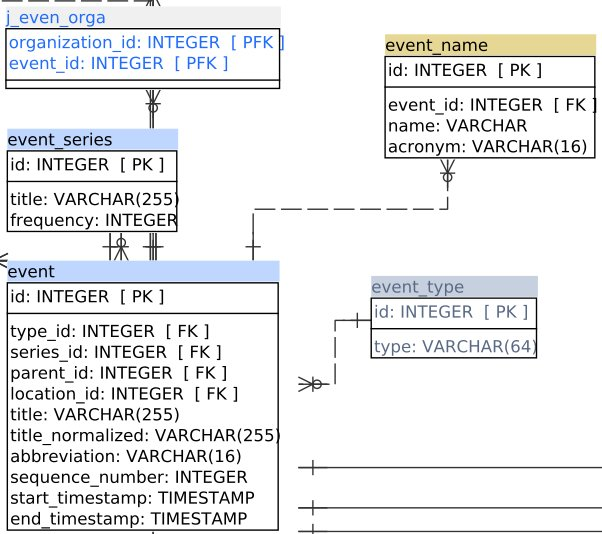
\includegraphics[width=6cm]{rrs_db_even.jpeg}
  \end{columns}
\end{frame}


\begin{frame}[containsverbatim]
  \frametitle{RRS: rozhraní k databázi}
  \begin{itemize}
    \item hlavní rozhraní
    \item je vstupem i výstupem všech modulů
  \end{itemize}
  \begingroup
  \fontsize{9pt}{11pt}\selectfont
  \begin{verbatim}
<event type="workshop">
  <title value="2008 USENIX Annual Technical Workshop"/>
  <from_timestamp value="2008-11-10"/>
  <to_timestamp value="2008-12-21"/>
  <location>
    <country value="USA"/>
    <city value="New York"/>
    <address value="767 Fifth Ave. New York City, 10153"/>
  </location>
</event>
  \end{verbatim}
  \endgroup
\end{frame}


% -----------------------------------------------------------------------------
% Vase projekty
% -----------------------------------------------------------------------------

\section {Va\v{s}e projekty}

\begin{frame}
  \frametitle{Vaše projekty}
  \begin{itemize}
    \item zadání
    \item \alert{\textbf{návrh, možnosti, výzkum}}
    \item implementace, ladění
    \item testování, výsledky
    \item odevzdání, ukončení projektu
  \end{itemize}
\end{frame}

\subsection{Vývojový cyklus projektu}
\begin{frame}
  \frametitle{Analýza, návrh, výzkum možností}
  \begin{itemize}
    \item orientace v tématu
    \item vyhledat si "jak se to dneska dělá"
    \item navrhnout nový způsob nebo zdokonalit stávající
    \item \alert{zde ještě nemáte napsanou ani čárku kódu}
    \item vyhledat vhodné knihovny, navrhnout skrukturu programu (UML...)
    \item \alert{zde stále ještě nemáte ani čárku kódu}
    \item začít programovat
  \end{itemize}
\end{frame}

\begin{frame}
  \frametitle{Implementace}
  \begin{itemize}
    \item Linux
    \item Python hacker? Ne! (dotaz)
    \item použití externích knihoven
    \item TDD? není nutností
    \item profiling (cProfile, timeit)
  \end{itemize}
\end{frame}

\begin{frame}
  \frametitle{Ladění na školních serverech}
  \begin{itemize}
    \item local, servery: athena1, athena2, athena3, pcknot1-6 (kill procesů!)
    \item Příkazy (system): source, nohup, ulimit, screen, top (dotaz)
    \item Nástroje (práce): grep, cut, less, touch, xmllint atp.
  \end{itemize}
\end{frame}

\begin{frame}
  \frametitle{Testování a vyhodnocení testů}
  \begin{itemize}
    \item Testování
    \begin{itemize}
      \item unit-testy
      \item dostatečně velká testovací sada
    \end{itemize}
    \item Vyhodnocení výsledků
    \begin{itemize}
      \item statistické hodnoty: úspěšnost (viz níže), čas, objem dat atp.
      \item slovní komentář (úspěchy, neúspěchy, možnosti dalšího  vývoje)
      \item samozřejmě popsat vše na wiki a README
    \end{itemize}
  \end{itemize}
  \begin{block}{Metriky (binární klasifikace)}
    \textbf{sensitivity, specificity, precission, recall, F-measure}
  \end{block}
\end{frame}


\subsection{Pravidla, štábní kultura}
\begin{frame}
  \frametitle{Štábní kultura}
  \begin{itemize}
    \item git
    \item komentáře, docstringy, epydoc, dodržovat PEPsy
    \item používejte Python jako skriptovací jazyk, ne jako C (C++)!
    \item Python - PascalCase class, lowercase\_underscored method
    \item modulární, objektový návrh (srovnej s Java – 1 class=1 file)
    \item adresářová struktura
    \item wiki – dle šablony
    \begin{itemize}
      \item \tiny{\textcolor{blue}{\underline{\href{https://merlin.fit.vutbr.cz/nlp-wiki/index.php/Rrs\_page\_template}{https://merlin.fit.vutbr.cz/nlp-wiki/index.php/Rrs\_page\_template}}}}
    \end{itemize}
    \item aktualizovaná data v repozitářích
  \end{itemize}
\end{frame}

\begin{frame}[containsverbatim]
  \frametitle{Doporučená adresářová struktura}
  \begin{itemize}
    \item /mnt/minerva1/nlp/projects/rrs\_******
    \item pozn.: pojmenovávání dokumentů - logicky! NE: init, main, test1, MyParser
  \end{itemize}
  \begingroup
  \fontsize{9pt}{11pt}\selectfont
  \begin{verbatim}
project_folder/
    backup/      zalohy
    bin/         spustitelne soubory (python, binarky..)
    doc/         generovana dokumentace (html, pdf)
    data/        schemata, sql, pomocne skripty, obrazky, xml
    git/         git repozitar
    input.test/  testovaci vstupy (XML)
    output.test/ testovaci vystupy (XML)
    tmp/         docasne soubory, odpad
    README.txt   kratky komentar k projektu, spusteni
    profile.sh   export promennych
  \end{verbatim}
  \endgroup
\end{frame}



\subsection{Dotazy a informace}
\begin{frame}
  \frametitle{Informace}
  \begin{itemize}
    \item \textcolor{blue}{Obecné:} https://merlin.fit.vutbr.cz/nlp-wiki/index.php/Rrs\_FAQ
    \item \textcolor{blue}{O RRS:} prakticky celá wiki, co začíná prefixem Rrs\_
    \item \textcolor{blue}{Metody:} Google, Google Scholar, CiteSeerX, Microsoft Academic Search
    \item \textcolor{blue}{Speciální:} mailem
    \begin{itemize}
      \item implementace, rozhraní, RRS, databáze - S. Heller
      \item organizační věci v projektu, ukončení, smlouvy atp. - Ing. Otrusina
      \item skoro nikdy - doc. Smrž
    \end{itemize}
  \end{itemize}
\end{frame}

\begin{frame}
  \frametitle{Dotazy e-mailem}
  \begin{itemize}
    \item něco mi v Pythonu nejde/nefunguje (odmítám odpovídat) - máte google, tutoriály...
    \item nevím co mám dělat: přečíst si znovu zadání, googlit, ptát se exaktně
    \item nefunkční knihovny (rrslib atp.):
    \begin{itemize}
      \item verze, (\textbf{git – revize!})
      \item popis problému
      \item \textbf{traceback} (dotaz)
    \end{itemize}
  \end{itemize}
\end{frame}

\subsection{Nástroje}
\begin{frame}
  \frametitle{Programová podpora, nástroje na školních serverech}
  \begin{itemize}
    \item athena3:/mnt/data2/rrs\_local/ - nejnovější
    \item athena2, pcknot : /mnt/minerva1/nlp/projects/rrs\_local/
    \item zkompilovaný Python 2.7.2, Ruby 1.9.2, knihovny (lxml, psycopg, \textbf{rrslib},
          \textbf{nltk}, chardet, nose, google-api, epydoc, Django, numpy, twisted)
  \end{itemize}
\end{frame}

\begin{frame}
  \frametitle{Rrslib}
  \begin{itemize}
    \item Pythoní knihovna vyvinutá pro účely projektu ReReSearch
    \item \textcolor{blue}{\underline{\href{https://merlin.fit.vutbr.cz/nlp-wiki/index.php/Rrs\_library}{https://merlin.fit.vutbr.cz/nlp-wiki/index.php/Rrs\_library}}}
    \item mimo KNOT Group není možné používat
    \item vzor
  \end{itemize}
  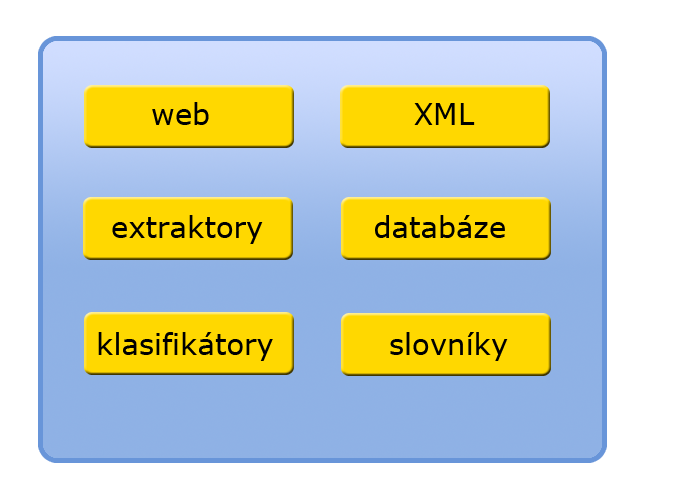
\includegraphics[width=5cm]{rrslib_structure.png}
\end{frame}

\begin{frame}
  \frametitle{Rrslib}
  \begin{description}
    \item[web -] {stahování stránek, parsery webových vyhledávačů, parser CSS}
    \item[extractors -] {hierarchie extraktorů (lokální dokumenty, web...), normalizace}
    \item[db -] {model DB, DBAL+ORM, import dat do DB}
    \item[dictionaries -] {efektivní implementace a API pro hledání}
    \item[classifiers -] {jazyk textu, úspěšnost převodu PDF do textu atp.}
    \item[xml -] {manipulace s formátem RRS-XML}
  \end{description}
\end{frame}

\begin{frame}[containsverbatim]
  \frametitle{Rrslib - příklad použití}
  {tutoriál - viz wiki}
  \begingroup
  \fontsize{6,5pt}{8pt}\selectfont
  \begin{verbatim}
>>> from rrslib.classifiers.language import LanguageIdentifier
>>> li
<rrslib.classifiers.language.LanguageIdentifier object at 0xb77de94c>
>>> s = "If you are a parent, like me, who has a boy you know how difficult it is"
>>> li.identify(s)
('english', 30.379752091537153)
>>>
>>> li.identify("Ahoj, ja jsem Jakub a mam rad vsechny lidi na tomto svete")
('czech', 25.314534512391173)
>>>
>>> li.identify("Ab sofort lässt sich auch die Leistung Ihres
mobilen Internetzugangs messen, zum Beispiel UMTS-Zugänge per
Notebook oder Internet-Verbindungen mit dem Handy...")
('german', 72.69410437330895)
  \end{verbatim}
  \endgroup
\end{frame}

\begin{frame}[containsverbatim]
  \frametitle{Rrslib - vývoj}
  \begin{itemize}
    \item rád přijmu šikovné devely do týmu
    \item http://athena3.fit.vutbr.cz:3000/projects/rrs-library/repository
  \end{itemize}
  \begingroup
  \fontsize{7pt}{8pt}\selectfont
  \begin{verbatim}
$ git clone xlogin00@merlin.fit.vutbr.cz:/mnt/minerva1/nlp/projects/\
  rrs_library/git-repository/rrslib.git
  \end{verbatim}
  \endgroup
\end{frame}

\begin{frame}
  \frametitle{nltk - natural language toolkit}
  \begin{itemize}
    \item Pythoní knihovna pro zpracování přirozeného jazyka
    \item tokenizery, parsery, CFG, taggery, stemmery, lemmatizér, klasifikátory
    \item extrakce informací z textu (NER - named entity recognition, relation extraction), ale poměrně slabá
    \item nainstalováno na athéně v rrs\_local
    \item \textcolor{blue}{\underline{\href{http://www.nltk.org/}{http://www.nltk.org/}}}
    \item \textcolor{blue}{\underline{\href{http://www.slideshare.net/japerk/nltk-in-20-minutes}{http://www.slideshare.net/japerk/nltk-in-20-minutes}}}
  \end{itemize}
\end{frame}

\begin{frame}
  \frametitle{Dotazy}
  \fontsize{25pt}{25pt}\selectfont{???}
\end{frame}

\end{document}

